\documentclass[11pt]{article}
\usepackage[margin=1in]{geometry}          
\usepackage{graphicx}
\usepackage{amsthm, amsmath, amssymb}
\usepackage{setspace}\onehalfspacing
\usepackage[loose,nice]{units} %replace "nice" by "ugly" for units in upright fractions
 \usepackage{breqn}
 \usepackage[cal=cm]{mathalfa}
 \usepackage{listings}

\title{Data Mining HW 1}
\author{Tobias Braun - tgb2117}
\date{Feb 19th 2019}

\begin{document}
\maketitle
\section*{Exercise 1}

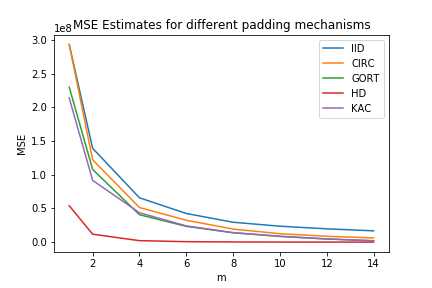
\includegraphics{MSE_Estimates.png}

When only considering the MSE of each dimensionality reduction method it appears
that IID is worst, then CIRC, then GORT, then KAC and the winner is the HD method 
using 3 HD blocks. One should always keep in mind that unbiasedness but even more 
so complexity are important factors when deciding which method to choose. 
Obviously, the accuracy of all estimators increases drastically with m and the 
MSE approaches 0 when m approaches d, which in our case is 16. But as the whole 
purpose of dimensionality reduction is to reduce m, this effect is not so much of
relevance when comparing different estimators.
\subsection*{Code}
\begin{lstlisting}
# -*- coding: utf-8 -*-
"""
Data Mining Homework 1 - dimensionality reduction

@author Tobias Braun, tgb2117
"""
################################imports########################################
import numpy as np
import matplotlib.pyplot as plt
import scipy as sp
import scipy.linalg as splin
np.random.seed(100)
############################prerequisites######################################
x_array = np.array(np.round_(np.random.rand(16)*100) - 50)
y_array = np.array(np.round_(np.random.rand(16)*100) - 50)

assert (np.abs(np.dot(x_array, y_array)) > 1)

################dimensionality reduction methods - definition##################
def IID (x: np.array, m: int, seed=100):
    np.random.seed(seed)
    G = np.random.normal(size=(m, np.shape(x)[0]))
    return np.matmul(G/np.sqrt(m), x)


def CIRC (x: np.array, m: int, seed=100):
    np.random.seed(seed)
    G = np.random.normal(size=(np.shape(x)[0]))
    CIRC = G
    for i in range(1, m):
        CIRC = np.vstack((CIRC, np.roll(G, 1)))
        G = np.roll(G, 1)
    return np.matmul(CIRC/np.sqrt(m), x)


def GORT (x: np.array, m: int, seed=100):
    np.random.seed(seed)
    G = np.random.normal(size=(np.shape(x)[0], m))
    GORT = np.transpose(np.linalg.qr(G)[0]*np.sqrt(np.shape(x)[0]))
    return np.matmul(GORT/np.sqrt(m), x)


def HD (x: np.array, m: int, seed=100):
    np.random.seed(seed)
    H = splin.hadamard(np.shape(x)[0])
    vec = np.random.choice([-1,1], np.shape(x)[0])
    D = np.diag(vec)
    vec_2 = np.random.choice([-1,1], np.shape(x)[0])
    D_2 = np.diag(vec_2)
    vec_3 = np.random.choice([-1,1], np.shape(x)[0])
    D_3 = np.diag(vec_3)
    
    HD_1 = np.matmul(H, D)
    HD_2 = np.matmul(H, D_2)
    HD_3 = np.matmul(H, D_3)
    HD_final = np.matmul(HD_1, HD_2)
    HD_final = np.matmul(HD_final, HD_3)/np.shape(x)[0]
    return np.matmul(HD_final/np.sqrt(m), x)

def KAC(x: np.array, m: int, seed=100):
    np.random.seed(seed)
    dim = np.shape(x)[0]
    no_of_givens = np.ceil(dim*np.log(dim))
    
    def givens (dim: int, seed=100):
        np.random.seed(seed)
        vec = np.repeat(1.0, dim)
        D = np.diag(vec)
        indices = np.random.choice(np.arange(0, dim), size=2, replace=False)
        i = np.amin(indices)
        j = np.amax(indices)
        theta = np.random.rand()*2*np.pi
        D[i][i] = np.cos(theta)
        D[i][j] = np.sin(theta)
        D[j][i] = -np.sin(theta)
        D[j][j] = np.cos(theta)
        return D
    
    multi_givens = [givens(dim, i) for i in np.random.choice(
            np.arange(0,100000), size=int(no_of_givens), replace=False)]
    pre_KAC = np.identity(dim)
    for i in range(0, len(multi_givens)):
        pre_KAC = np.matmul(pre_KAC, multi_givens[i])
        
    indices = np.random.choice(np.arange(0, dim), size=m, replace=False)
    KAC = np.sqrt(dim)*pre_KAC[indices]
    
    return np.matmul(KAC/np.sqrt(m), x)
    

###############dimensionality reduction methods - MSE testing##################

true_kernel_value = np.dot(x_array, y_array)
m_ = [1,2,4,6,8,10,12,14]

def MSE_Estimate_IID(x: np.array, y: np.array, m: int):
    iid = 0
    for i in range(0,1000):
        x_red = IID(x, m, i)
        y_red = IID(y, m, i)
        kernel_after_d_reduction = np.dot(x_red, y_red)
        sq_diff = np.power(kernel_after_d_reduction - true_kernel_value, 2)
        iid += sq_diff
        
    MSE_estimate = iid/1000
    return MSE_estimate

IID_MSE_Estimate = [MSE_Estimate_IID(x_array, y_array, m) for m in m_]

def MSE_Estimate_CIRC(x: np.array, y: np.array, m: int):
    circ = 0
    for i in range(0,1000):
        x_red = CIRC(x, m, i)
        y_red = CIRC(y, m, i)
        kernel_after_d_reduction = np.dot(x_red, y_red)
        sq_diff = np.power(kernel_after_d_reduction - true_kernel_value, 2)
        circ += sq_diff
        
    MSE_estimate = circ/1000
    return MSE_estimate

CIRC_MSE_Estimate = [MSE_Estimate_CIRC(x_array, y_array, m) for m in m_]

def MSE_Estimate_GORT(x: np.array, y: np.array, m: int):
    gort = 0
    for i in range(0,1000):
        x_red = GORT(x, m, i)
        y_red = GORT(y, m, i)
        kernel_after_d_reduction = np.dot(x_red, y_red)
        sq_diff = np.power(kernel_after_d_reduction - true_kernel_value, 2)
        gort += sq_diff
        
    MSE_estimate = gort/1000
    return MSE_estimate

GORT_MSE_Estimate = [MSE_Estimate_GORT(x_array, y_array, m) for m in m_]

def MSE_Estimate_HD(x: np.array, y: np.array, m: int):
    hd = 0
    for i in range(0,1000):
        x_red = HD(x, m, i)
        y_red = HD(y, m, i)
        kernel_after_d_reduction = np.dot(x_red, y_red)
        sq_diff = np.power(kernel_after_d_reduction - true_kernel_value, 2)
        hd += sq_diff
        
    MSE_estimate = hd/1000
    return MSE_estimate

HD_MSE_Estimate = [MSE_Estimate_HD(x_array, y_array, m) for m in m_]

def MSE_Estimate_KAC(x: np.array, y: np.array, m: int):
    kac = 0
    for i in range(0,1000):
        x_red = KAC(x, m, i)
        y_red = KAC(y, m, i)
        kernel_after_d_reduction = np.dot(x_red, y_red)
        sq_diff = np.power(kernel_after_d_reduction - true_kernel_value, 2)
        kac += sq_diff
        
    MSE_estimate = kac/1000
    return MSE_estimate

KAC_MSE_Estimate = [MSE_Estimate_KAC(x_array, y_array, m) for m in m_]


IID_ = plt.plot(m_, IID_MSE_Estimate, label='IID')
CIRC_ = plt.plot(m_, CIRC_MSE_Estimate, label='CIRC')
GORT_ = plt.plot(m_, GORT_MSE_Estimate, label='GORT')
HD_ = plt.plot(m_, HD_MSE_Estimate, label='HD')
KAC_ = plt.plot(m_, KAC_MSE_Estimate, label='KAC')
plt.legend()
plt.title("MSE Estimates for different padding mechanisms")
plt.xlabel("m")
plt.ylabel("MSE")
#plt.savefig('MSE_Estimates.png')
plt.show()
\end{lstlisting}

\section*{Exercise 2}

We know that the isotropic Gaussian kernel of the form \(K : \mathbb{R}^d \times \mathbb{R}^d \rightarrow \mathbb{R}$ defined as: 
\begin{equation*}
k(\mathbf{x},\mathbf{y}) = e^{- \frac{\lVert \tau \rVert^2}{2}}
\end {equation*}
is a special subclass of the nonisotropic Gaussian kernels with covariance matrix $Q = \mathcal{I}$ (where $\mathcal{I}$ denotes the identity matrix of corresponding dimension m) and can be approximated with the help of random feature maps as follows:
\begin{equation*}
\hat{K}_{base}(x,y) = \Phi(x) \times \Phi(y), \quad \text{with} \quad  \Phi(z) = 
\begin{bmatrix}
          \cos(\omega_1^Tz_1) \\
          \cos(\omega_2^Tz_2) \\
          \vdots \\
          \cos(\omega_m^Tz_m)\\
          \sin(\omega_1^Tz_1) \\
          \sin(\omega_2^Tz_2) \\
          \vdots \\
          \sin(\omega_m^Tz_m)
         \end{bmatrix}
\end {equation*}
We also know that the matrix $Q$ in non-isotropic Gaussian kernels is positive semi-definite and symmetrical as it is a covariance matrix. We can make use of this fact to construct a transformation of any non-isotropic Gaussian kernel into an isotropic Gaussian kernel. \newline
First, we decompose matrix Q such that $Q = V^TV$ as follows:
\begin{equation*}
Q = YDY^T
\end {equation*}
This decomposition, also called "eigendecomposition", is always possible for symmetric matrices as they are diagonalizable. The columns of Y are the eigenvectors of $Q$ and the diagonal entries of $D$ are the eigenvalues of $Q$. \newline
Because $Q$ is positive semi-definite, all entries in $D$ are positive and $Q$ can be rewritten as:
\begin{equation*}
Q = YDY^T=YD^{\frac{1}{2}}D^{\frac{1}{2}T}Y^T=YD^{\frac{1}{2}}(YD^{\frac{1}{2}})^T
\end {equation*}
Let $V= (D^{\frac{1}{2}}Y)^T$, then $Q=V^TV$ and subsequently:
\begin{equation*}
e^{-\frac{\tau^TQ\tau}{2}} = e^{-\frac{\tau^TV^TV\tau}{2}}
\end {equation*}
If we now define $f(z)$ as $f(z)=(YD^{\frac{1}{2}})^Tz$ and similarly $f(z^T)=z^T(YD^{\frac{1}{2}})$ and $\lambda$ as $\lambda = f(\tau)$ and $\lambda^T$ as $\lambda^T = f(\tau^T)$, then we obtain the following equality:
\begin{equation*}
e^{-\frac{\tau^TQ\tau}{2}} = e^{-\frac{\lambda^T \lambda}{2}} = e^{- \frac{\lVert \lambda \rVert^2}{2}}
\end {equation*}
The above transformation transforms any non-isotropic kernel into an isotropic one. 
Lastly, to improve the accuracy of our estimated kernel, we make use of Gaussian orthogonal matrices $G_{ort}$ instead of unstructured Gaussian matrices $G$. $G_{ort}$ is computed from $G$ by Gram-Schmidt orthogonalization and rescaling of the orthogonalized matrix with factor $\sqrt{m}$ such that the length of each row is equivalent to that of an unstructured Gaussian matrix (it is assumed that after Gram-Schmidt orthogonalization the rows are normalized to length 1).
Concluding, the kernel approximation for non-isotropic kernels is the following:
\begin{dmath*}
\hat{K}_{ort, noniso}(x,y) = \frac{1}{m} \sum_{i=1}^{m} \cos(\sqrt{m} \omega_{i,ort}^T(f(x-y)) =  \frac{1}{m} \sum_{i=1}^{m} \cos[\sqrt{m} \omega_{i,ort}^T(YD^{\frac{1}{2}})^Tx-(YD^{\frac{1}{2}})^Ty)] =   \frac{1}{m} \sum_{i=1}^{m}\{ \cos[\sqrt{m}\omega_{i,ort}^T(YD^{\frac{1}{2}})^Tx]\cos[\sqrt{m}\omega_{i,ort}^T(YD^{\frac{1}{2}})^Ty]+ \sin[\sqrt{m}\omega_{i,ort}^T(YD^{\frac{1}{2}})^Tx]\sin[\sqrt{m}\omega_{i,ort}^T(YD^{\frac{1}{2}})^Ty]\}
\end{dmath*}
where $\omega_{i,ort}$ are vectors sampled from $G_{ort}$.\newline
The above defined function $\Phi(z)$  changes correspondingly to $\Phi_{ort, noniso}(z)$:

\begin{equation*}
\hat{K}_{ort, noniso}(x,y) = \Phi_{ort, noniso}(x) \times \Phi_{ort, noniso}(y), \quad \text{with} \quad \Phi_{ort, noniso}(z) = 
\begin{bmatrix}
	
          \cos[\sqrt{m}\omega_{1,ort}^T(YD^{\frac{1}{2}})^Tz_1] \\
          \cos[\sqrt{m}\omega_{2,ort}^T(YD^{\frac{1}{2}})^Tz_2] \\
          \vdots \\
           \cos[\sqrt{m}\omega_{m,ort}^T(YD^{\frac{1}{2}})^Tz_m] \\
          \sin[\sqrt{m}\omega_{1,ort}^T(YD^{\frac{1}{2}})^Tz_1] \\
          \sin[\sqrt{m}\omega_{2,ort}^T(YD^{\frac{1}{2}})^Tz_2] \\
          \vdots \\
          \sin[\sqrt{m}\omega_{m,ort}^T(YD^{\frac{1}{2}})^Tz_m] 
         \end{bmatrix}
\end {equation*}
When looking at the complexity of this operation Victor Y. Pan, Zhao Q. Chen found in "The Complexity of the Matrix Eigenproblem" in STOC 1999: 507-516 that eigenvalue decomposition can be achieved in $O(n^3+n^2\log^2(n)\log(b))$ time, where the eigenvalues are approximated to within $2^{-b}$ accuracy. Apart from the decomposition, the Gram-Schmidt orthogonalization is the most computational demanding with a complexity of $O(m^3)$ as the process must be applied $m$ times and each orthogonalization takes $O(m^2)$ operations (multiplications and additions). Thus, the overall time complexity will be in the realms of $O(m^3)$ for vectors of dimension $m$ with corresponding covariance matrix of dimension $m \times m$.
\end{document}
